\addcontentsline{toc}{section}{Introduction}
\section*{Introduction}
L’identification par biométrie vocale est le processus de reconnaissance et de vérification de l’identité d’une personne à partir de leur enregistrement vocal. Elle a des applications importantes telles que la sécurité a criminalistique, l’IoT, les centres d’appel, et l’interaction homme-machine. Elle a été révolutionnée par les techniques d’apprentissage profond ces dernières années, permettant une identification plus précise, même dans des environnements acoustiques difficiles avec des parasites sonores. Ces techniques exploitent de grandes quantités de données vocales pour former des modèles de réseaux neuronaux qui peuvent apprendre à extraire automatiquement des caractéristiques discriminantes des signaux vocaux.

Dans ce chapitre, nous clarifierons d’abord les concepts clés liés à notre étude. Par la suite nous présenterons les quelques techniques de mise en place de ce type de modèles d’Intelligence Artificielle.

\section{Définitions}
\subsection{Biométrie}

La biométrie comprend tout un ensemble de technologies et procédés de reconnaissance, d’authentification et d’identification des personnes à partir de certaines de leurs caractéristiques physiques (empreintes digitales, la forme de la main, du doigt, le réseau veineux, l'œil), biologiques (ADN, le sang, la salive) ou comportementales (reconnaissance vocale, la dynamique des signatures). Ces caractéristiques doivent être à la fois \cite{idemia} :	
\begin{itemize}
    \item Universelles : pour être utilisables par tous ; 
    \item Uniques : pour distinguer les personnes sans équivoque;
    \item Invariables : pour permettre une utilisation tout au long de la vie;
    \item Mesurables : pour permettre la comparaison.
\end{itemize}

Les différentes techniques utilisées font l'objet de recherches régulières, de développements et bien entendu, d'améliorations constantes.
Toutefois, les différentes sortes de mesures n'ont pas le même niveau de fiabilité.
On estime que les mesures physiologiques ont l'avantage d'être plus stables dans la vie d'un individu.
Par exemple, elles ne subissent pas autant les effets du stress, contrairement à l'identification par mesure comportementale \cite{idemia}.

\subsection{Biométrie vocale}
l'authentification par Biométrie vocale consiste à utiliser la voix d'une personne comme caractéristique biologique d'identification unique afin de l'authentifier.
La Biométrie vocale est considérée comme la méthode d'authentification la plus solide car elle lie l'identité à un individu réel \textbf{("ce que vous êtes" plutôt que "ce que vous savez" ou "ce que vous avez")}.
Elle  extrait un ensemble de caractéristiques audio qui garantissent qu'un locuteur est une personne réelle plutôt qu'un enregistrement ou un synthétique voix d'un individu \cite{nice}.
%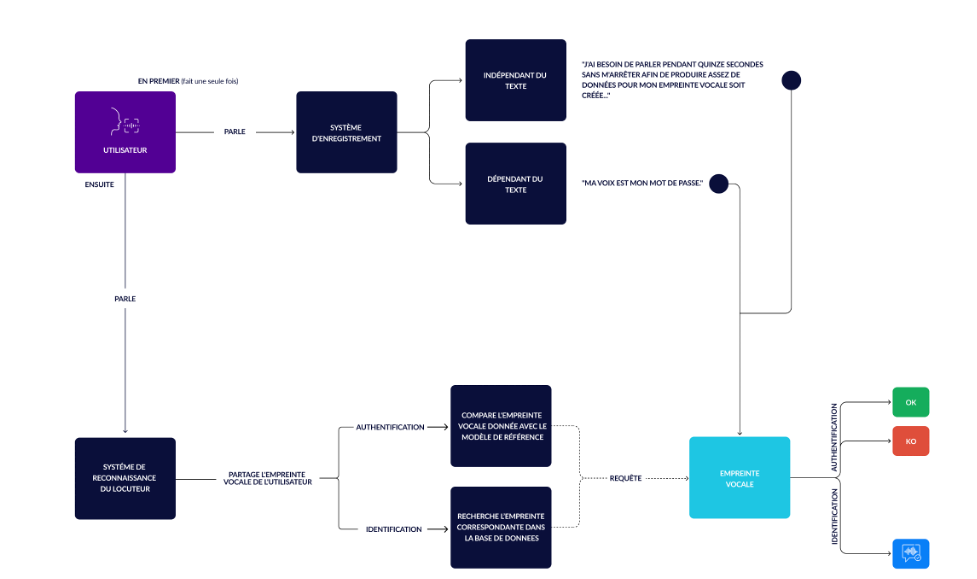
\includegraphics{1-Picture1}  
%1-Picture1.png
\begin{figure}[ht]
    \centering
    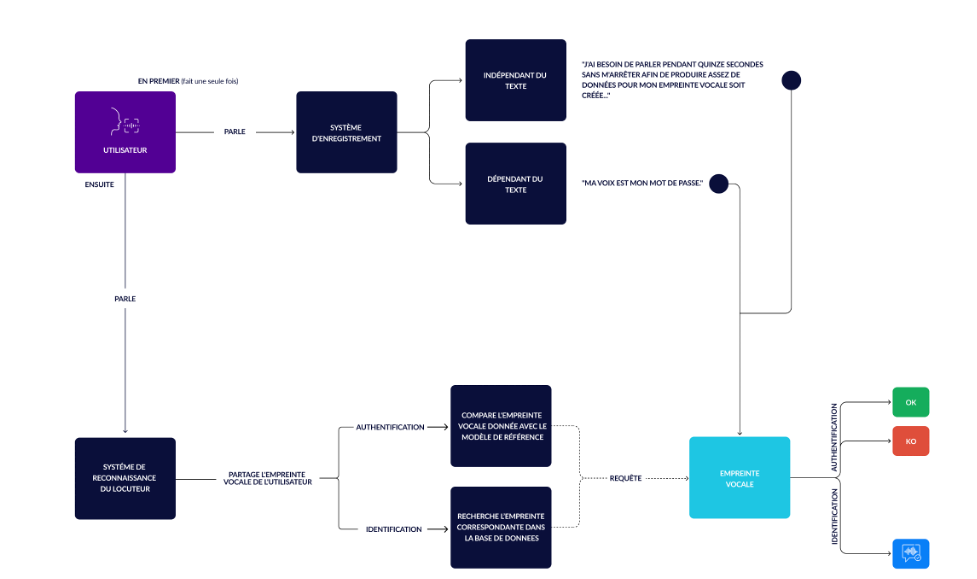
\includegraphics[width=1\textwidth]{1-Picture1}
    \caption{Architecture d'une IA de reconnaissance par biométrie vocale.}
    \label{fig:1-Picture1}
    \source{Source of the image.}
\end{figure}

\subsection{Identification et authentification biométrique}
La biométrie permet l'identification et l'authentification d'une personne à partir de données reconnaissables et vérifiables, qui lui sont propres et qui sont uniques.
\paragraph{}\textbf{L'identification }consiste à déterminer l'identité d'une personne.
Il s'agit de saisir une donnée biométrique de cette personne, en prenant par exemple une photo de son visage, en enregistrant sa voix, ou en captant l'image de son empreinte digitale. Ces données sont ensuite comparées aux données biométriques de plusieurs autres personnes qui figurent dans une base; \textbf{ ici, on essaye de répondre à la question: « qui êtes-vous ? »}.
\paragraph{}\textbf{L'authentification}, appelée également vérification, est le processus qui consiste à comparer les données caractéristiques provenant d'une personne, au modèle de référence biométrique de cette dernière (« template »), afin de déterminer la ressemblance. Le modèle de référence est préalablement enregistré et stocké dans une base de données, dans un équipement ou objet personnel sécurisé. On vérifie ici que la personne présentée est bien la personne qu'elle prétend être.
Dans ce cas on essaye de répondre à la question: « êtes-vous bien celui que vous prétendez être ? ».
\subsection {Deep learning}
\textbf{Le deep learning ou apprentissage profond}  est une technique d'apprentissage automatique basée sur des réseaux de neurones artificiels. Dans le domaine de la reconnaissance vocale, l'apprentissage profond est largement utilisé pour améliorer la précision de la reconnaissance \cite{embeddings}.


\section{historique de la biométrie vocale}
La biométrie répond à une préoccupation très ancienne de prouver son identité, de manière irréfutable, et en utilisant nos différences et particularités.
\paragraph{}\textbf{1952}: le premier système de reconnaissance vocale a été développé par Lawrence G. Roberts et ses collègues au laboratoire Lincoln du MIT. Le système utilisait l’analyse spectrographique de fichiers vocaux comparé á une base de données de d’empreintes vocales de personnes bien identifiées.
\paragraph{}\textbf{1962}: les laboratoires Bell ont créé le système "voiceprint", qui utilise un spectrogramme pour analyser les modèles de fréquence uniques de la voix d’un locuteur afin de les identifier. 
\paragraph{}\textbf{Années 1970}: Plusieurs systèmes d’identification de d’individus par empreinte vocale commerciaux ont été développés, y compris le système VeriVox de Raytheon et le système VoiceID de Bolt Beranek et Newman (BBN).
\paragraph{}\textbf{Années 1990}: Les chercheurs ont commencé à explorer l’utilisation de réseaux neuronaux pour l’identification des individus par voix, ce qui a permis une identification plus précise et plus fiable.
\paragraph{}\textbf{Années 2000}: L’identification des individus par voix est devenue plus largement utilisée dans les applications d’application de la loi et de sécurité, et les chercheurs ont commencé à explorer l’utilisation d’algorithmes d’apprentissage automatique pour identifier automatiquement les locuteurs sans avoir besoin d’une base de données préexistante de locuteurs connus. 
\paragraph{}Aujourd’hui, l’identification des individus par voix continue d’être un domaine de recherche actif, avec des applications dans divers domaines, notamment l’application de la loi, la sécurité et la criminalistique.


\section{Types de reconnaissances vocales}
Les principes de la biométrie vocale sont généralement séparés en 2 types :
\begin{itemize}
    \item Dépendant du texte : \\Ce type de reconnaissance du locuteur exige que l’utilisateur dise exactement l’expression enregistré. Cela manque de flexibilité étant donné que l’utilisateur doit se souvenir de ladite expression, mais offre une précision et une rapidité intéressantes.
    \item Independant du texte : \\Ce processus de vérification n’a pas la contrainte de contenu. L’utilisateur peut parler librement. Toutefois, l’entraînement et les tests d’énonciation prendront plus de temps pour atteindre la performance attendue \cite{timedoctor}.
\end{itemize}

\section{Fonctionnement}
La Biométrie vocale utilise des modèles de voix pour générer une identification unique pour chaque individu, en travaillant avec plus de 100 caractéristiques physiques et comportementales. Il comprend la vitesse de la parole, l'accent, la prononciation, l'emphase, en plus des facteurs physiques de vos voies vocales, de votre bouche et de vos voies nasales \cite{imageware}.

\begin{figure}[h]
    \centering
    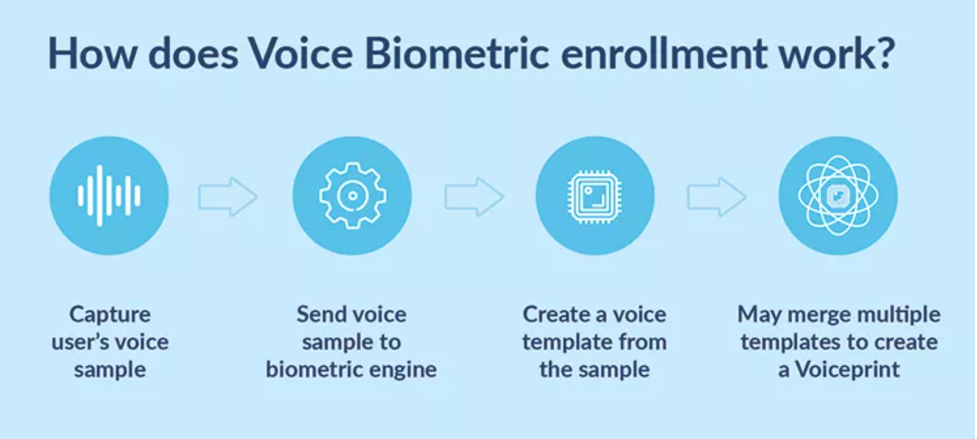
\includegraphics[width=1\textwidth]{2-fonctionnement}
    \caption{Ajout d'un individu à une IA de reconnaissance parempreinte vocale.}
    \label{fig:2-fonctionnement}
\end{figure}

Selon la méthode d’authentification (dépendante du texte ou indépendante du texte), une IA de biométrie vocale collecte le modèle vocal d’un utilisateur \cite{rcdevs}. Cependant, il n’authentifie pas ce que l’utilisateur dit. Il vérifie seulement qui parle.
Il extrait les caractéristiques qui distinguent le discours d’une personne des autres. Le résultat est une empreinte vocale ou un modèle vocal, tel qu’on peut avoir une empreinte digitale.  
Cela signifie-t-il qu’une personne avec une voix similaire peut contourner le système?
La voix d’une personne est extrêmement difficile à forger à des fins de comparaison biométrique en raison de son caractère unique inhérent comme le dialecte, le style de parole etc. 

Cela signifie simplement que même si une usurpation d’identité vocale est ressemblant pour une oreille humaine, une analyse détaillée de l’empreinte vocale effectuée à l’aide d’algorithmes informatiques peut aider à la distinguer de l’échantillon.
Cela grâce a Plus de 100 caractéristiques physiques du corps, chacune avec une taille et une forme unique, qui contribuent à la façon dont une personne parle. 
La biométrie vocale repose sur des caractéristiques vocales fortement corrélées aux qualités physiologiques de la façon dont une personne crée la parole.  
Maintenant que nous avons étudié l’authentification vocale et son fonctionnement, jetons un coup d’œil à certaines de ses applications réelles.


\section{cas d’utilisation de la biométrie vocale}
\paragraph{}Des centres d’appel (call center), et des applications mobiles aux applications de messagerie et aux appareils domotiques intelligents, la biométrie vocale peut fonctionner dans divers cas d'utilisation  \cite{vivoka}.

Voici un aperçu détaillé de ceux-ci :
\begin{itemize}
    \item les applications mobiles :\\Le principal cas d'utilisation de l'authentification vocale auprès des consommateurs est l'authentification mobile mains libres. Tout ce que vous avez à faire est de fournir une commande vocale pour vous connecter ou autoriser les achats, éliminant ainsi le besoin de mémoriser les identifiants et les mots de passe.
    Ceci est idéal pour les téléphones portables ou d'autres paramètres où la reconnaissance faciale et d'autres formes d'authentification biométrique peuvent être gênantes.
    De plus, l'authentification vocale peut également être utile pour les solutions d'assistant virtuel telles que Google Home, Alexa d'Amazon et Siri. On peut l'utiliser pour passer des commandes et effectuer d'autres fonctions qui nécessitent une certaine authentification.
    
    \item les Centres d'appels et systèmes IVR(Interactive Voice Response):\\Les méthodes de sécurité obsolètes comme les mots de passe traditionnels ou les questions ne sont plus suffisamment sécurisées.
    Les systèmes de biométrie vocale offrent une résistance contre l'imitation de la voix grâce à des algorithmes intrinsèques utilisés pour l'analyse biométrique et offrent une liste de blocage. Cela rend la technologie particulièrement utile dans le secteur de l'assistance téléphonique.
    On peut également utiliser la reconnaissance vocale comme authentificateur lors des appels d'assistance client. Les appelants peuvent trouver cela plus pratique et plus sûr que de partager des données personnelles telles que leur numéro de licence ou de carte de crédit à des fins de vérification d'identité.
    
    \item les Applications web:\\On peut ajouter des systèmes de vérification vocale à des pages Web ou à des applications dans les secteurs de la banque et du commerce électronique. L'authentification vocale dans les applications Web peut être utile pour l'identification à distance des utilisateurs.
    De plus, l'inscription passive ou l'authentification indépendante du texte facilite l'intégration de nouveaux utilisateurs pour votre service sans aucune inscription. Les clients sont automatiquement vérifiés en temps réel lorsqu'ils interagissent avec un agent IVR ou un centre de contact.
    
    \item Les objetc connectés:\\Les applications IoT offrent des moyens nouveaux et innovants de communication et d'interaction entre les humains et les machines.
    Une mise en œuvre appropriée de l'authentification vocale peut offrir une expérience utilisateur plus flexible que les méthodes traditionnelles telles que les écrans tactiles.
    Et comme l'authentification vocale peut fournir une couche de sécurité supplémentaire, vous pouvez facilement accéder à votre appareil domotique IoT sans aucun souci.
    De toute évidence, l'authentification biométrique vocale semble rendre les choses beaucoup plus faciles.
    Cependant, avant de décider d'utiliser l'authentification vocale pour votre entreprise, examinons ses avantages et ses défis \cite{thalesgroup}.
    
\end{itemize}

\section{Les avantages de la biométrie vocale}
La Biométrie vocale peut être utilisé dans le cadre d'un processus d'authentification à deux facteurs pour augmenter la sécurité et les 3 principaux avantages sont :
\begin{itemize}
    \item Améliorer l'expérience client avec une authentification rapide et fluide
    \item Améliorer la sécurité et minimiser les violations dues aux mots de passe compromis, au phishing, etc…
    \item Identifier instantanément les utilisateurs et personnalisez l'interaction. Grâce à la technologie de Biométrie vocale, les appelants n'ont plus besoin de fournir de mots de passe ou de codes PIN ni de répondre à des questions de sécurité pour vérifier leur identité. Cela rend la biométrie vocale idéale pour les déploiements multicanaux. Une fois qu'un utilisateur est inscrit, on peut utiliser son empreinte vocale sur tous les canaux d'assistance d’une organisation \cite{timedoctor}.
\end{itemize}


\section{Les inconveninents de la biométrie vocale}
%La Biométrie vocale peut être utilisé dans le cadre d'un processus d'authentification à deux facteurs pour augmenter la sécurité et les 3 principaux avantages sont :
\begin{itemize}
    \item Authentification via des contrefaçons audio:\\Les récents progrès de la technologie ont permis aux gens de créer des contrefaçons profondes. Il s'agit de fausses voix produites synthétiquement d'une personne, identiques à leur voix d'origine.
    Les contrefaçons profondes sont de plus en plus courantes et peuvent faire croire à un programme d'IA en son authenticité.
    Alors, comment empêcher les utilisateurs non autorisés d'entrer dans la base de données ?
    Vous pouvez créer une liste d'autorisation d'empreintes vocales et les stocker dans un répertoire actif. Au cours de ce processus, le système de reconnaissance vocale inscrit l'utilisateur dans une liste de membres autorisés.
    Ainsi, chaque fois qu'un utilisateur essaie d'accéder au système, son empreinte vocale est comparée à la fois à la liste d'autorisation et à une liste de blocage des empreintes vocales des fraudeurs .
    Et pendant que l'authentification est en cours, la détection passive des fraudes peut envoyer des alertes si l'empreinte vocale correspond à la base de données de la liste noire. 
    
    \item Manque de précision:\\Le bruit de fond ou son parasite est l'un des principaux facteurs qui affectent la reconnaissance automatique de la parole. Cela peut avoir un impact sur la qualité du modèle de voix de l'orateur et, à son tour, diminuer le niveau de précision du processus d'authentification.
    Un système d'authentification vocale peut ne pas être en mesure de faire la différence entre le discours de l’utilisateur, les autres personnes qui parlent et le bruit ambiant, ce qui entraîne des confusions et des erreurs  \cite{aware}.
    \\Cela signifie qu'il peut être difficile d'utiliser l'authentification vocale dans des environnements bruyants tels que des bureaux très fréquentés ou des espaces publics.
    \\Pour une authentification transparente, on peut utiliser des microphones proches ou des casques antibruit qui permettent au logiciel de se concentrer sur le discours de l’utilisateur. 
    \\L'identification du locuteur est le processus de détermination de l'identité d'une personne en fonction de sa voix. Il s'agit d'une tâche essentielle dans de nombreuses applications, y compris l'application de la loi, la sécurité et la reconnaissance vocale.
    \\L'état de l'art en matière d'identification du locuteur implique l'utilisation de techniques d'apprentissage en profondeur, qui ont considérablement amélioré la précision et la fiabilité du processus. Les modèles d'apprentissage en profondeur les plus populaires pour l'identification du locuteur comprennent les réseaux de neurones convolutifs (CNN), les réseaux de neurones récurrents (RNN) et leurs variantes.
    \\L'un des principaux défis de l'identification du locuteur est de gérer la variabilité des signaux vocaux. Des facteurs tels que le bruit de fond, l'accent et l'état émotionnel peuvent affecter de manière significative la qualité des signaux vocaux, ce qui rend difficile l'identification précise du locuteur. Pour relever ce défi, les chercheurs ont développé diverses techniques d'extraction de caractéristiques, telles que les coefficients cepstraux de fréquence Mel (MFCC), qui sont couramment utilisés dans le traitement de la parole.
    \\Ces dernières années, les chercheurs ont également exploré l'utilisation d'autres modalités biométriques, telles que la reconnaissance faciale et la reconnaissance de l'iris, en conjonction avec l'identification du locuteur pour améliorer la précision globale du processus. Ces approches multimodales tirent parti des atouts de différentes modalités biométriques pour améliorer le processus d'identification.
    \\Dans l'ensemble, l'état de l'art en matière d'identification des locuteurs continue d'évoluer rapidement, les recherches en cours se concentrant sur le développement de modèles plus robustes et plus précis pour identifier les locuteurs dans des environnements difficiles.
\end{itemize}

\section{Apprenttissage profond}
\subsection{Notion d’IA} 
\paragraph{}L'intelligence artificielle est née dans les années 1950, lorsqu'une poignée de pionniers du domaine naissant de l'informatique ont commencé à se demander si les ordinateurs pouvaient être amenés à "penser" - une question dont nous explorons encore les ramifications aujourd'hui. Une définition concise du domaine serait la suivante : l'effort d'automatisation des tâches intellectuelles normalement exécutées par les humains. En tant que tel, l'IA est un domaine général qui englobe l'apprentissage automatique et l'apprentissage en profondeur, mais qui comprend également de nombreuses autres approches qui n'impliquent aucun apprentissage. Les premiers programmes d'échecs, par exemple, n'impliquaient que des règles codées en dur conçues par des programmeurs et n'étaient pas considérées comme de l'apprentissage automatique. 
\paragraph{}Pendant assez longtemps, de nombreux experts ont cru que l'intelligence artificielle au niveau humain pouvait être obtenue en demandant aux programmeurs de créer à la main un ensemble suffisamment large de règles explicites pour manipuler les connaissances. Cette approche est connue sous le nom d'IA symbolique et a été le paradigme dominant de l'IA des années 1950 à la fin des années 1980. Il a atteint son apogée pendant le boom des systèmes experts des années 1980.
\paragraph{}Bien que l'IA symbolique se soit avérée adaptée pour résoudre des problèmes logiques bien définis, comme jouer aux échecs, il s'est avéré impossible de trouver des règles explicites pour résoudre des problèmes plus complexes et flous, tels que la classification d'images, la reconnaissance vocale et le langage. Une nouvelle approche est apparue pour prendre la place symbolique de l'IA : l'apprentissage automatique.


\begin{figure}[h]
    \centering
    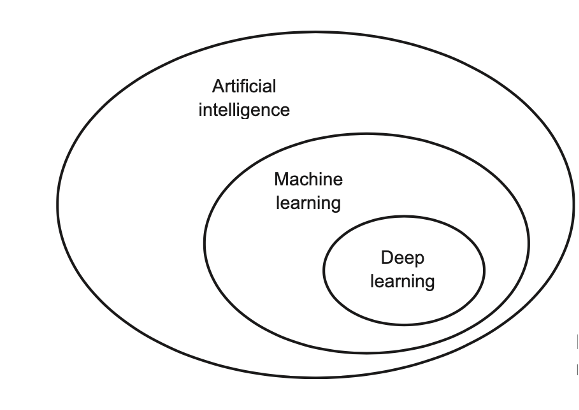
\includegraphics[width=1\textwidth]{1-ia-ml-dl}
    \caption{Intelligence Artificielle, Machin learning et Deep learning.}
    \label{fig:1-ia-ml-dl}
\end{figure}

\subsection{Notion d'apprentissage automatique}
\paragraph{}Dans l'Angleterre victorienne, Lady Ada Lovelace était une amie et collaboratrice de Charles Babbage, l'inventeur de la machine analytique : le premier ordinateur mécanique polyvalent connu. Bien que visionnaire et très en avance sur son temps, l'Analytical Engine n'était pas conçu comme un ordinateur à usage général lorsqu'il a été conçu dans les années 1830 et 1840, car le concept de calcul à usage général n'était pas encore inventé. Il s'agissait simplement d'un moyen d'utiliser des opérations mécaniques pour automatiser certains calculs du domaine de l'analyse mathématique, d'où le nom de moteur analytique. 
\paragraph{}En 1843, Ada Lovelace a fait remarquer à propos de l'invention : « La machine analytique n'a aucune prétention à créer quoi que ce soit. Il peut faire tout ce que nous savons comment lui ordonner de fonctionner... Son rôle est de nous aider à mettre à disposition ce que nous connaissons déjà. Cette remarque a ensuite été citée par le pionnier de l'IA, Alan Turing, comme "l'objection de Lady Lovelace" dans son article historique de 1950 "Computing Machinery and Intelligence",1 qui a présenté le test de Turing ainsi que les concepts clés qui allaient façonner l'IA. Turing citait Ada Lovelace alors qu'il se demandait si les ordinateurs à usage général pouvaient être capables d'apprentissage et d'originalité, et il en est venu à la conclusion qu'ils le pouvaient.
\paragraph{}L'apprentissage automatique découle de cette question : un ordinateur pourrait-il aller au-delà de "ce que nous savons lui ordonner d'exécuter" et apprendre par lui-même comment effectuer une tâche spécifiée ? Un ordinateur pourrait-il nous surprendre ? Plutôt que des programmeurs élaborant des règles de traitement de données à la main, un ordinateur pourrait-il automatiquement apprendre ces règles en examinant les données ?
Cette question ouvre la porte à un nouveau paradigme de programmation. 
\paragraph{}En programmation classique, le paradigme de l'IA symbolique, les humains saisissent des règles (un programme) et des données à traiter selon ces règles, et en sortent des réponses (voir figure 1.2).
\paragraph{}Avec l'apprentissage automatique, les humains saisissent les données ainsi que les réponses attendues des données, et sortent les règles. Ces règles peuvent ensuite être appliquées à de nouvelles données pour produire des réponses originales.

\begin{figure}[h]
    \centering
    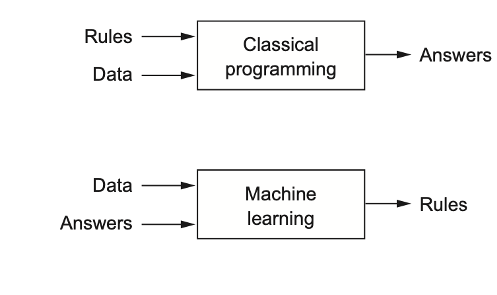
\includegraphics[width=1\textwidth]{1-ml}
    \caption{Machin learning Nouveau paradigme de programmation.}
    \label{fig:1-ml}
\end{figure}

\paragraph{}Un système d'apprentissage automatique est entraîné plutôt qu'explicitement programmé. Il est présenté avec de nombreux exemples pertinents pour une tâche, et il trouve une structure statistique dans ces exemples qui permet finalement au système de proposer des règles pour automatiser la tâche. 
\paragraph{}Par exemple, si vous souhaitez automatiser la tâche d'étiquetage de vos photos de vacances, vous pouvez présenter un système d'apprentissage automatique avec de nombreux exemples d'images déjà étiquetées par des humains, et le système apprendrait des règles statistiques pour associer des images spécifiques à des étiquettes spécifiques.
\paragraph{}Un système d'apprentissage automatique est entraîné plutôt qu'explicitement programmé. Il est présenté avec de nombreux exemples pertinents pour une tâche, et il trouve une structure statistique dans ces exemples qui permet finalement au système de proposer des règles pour automatiser la tâche. Par exemple, si vous souhaitez automatiser la tâche d'étiquetage de vos photos de vacances, vous pouvez présenter un système d'apprentissage automatique avec de nombreux exemples d'images déjà étiquetées par des humains, et le système apprendrait des règles statistiques pour associer des images spécifiques à des étiquettes spécifiques.
\paragraph{}Bien que l'apprentissage automatique n'ait commencé à prospérer que dans les années 1990, il est rapidement devenu le sous-domaine de l'IA le plus populaire et le plus réussi, une tendance stimulée par la disponibilité d'un matériel plus rapide et d'ensembles de données plus volumineux. 
\paragraph{}L'apprentissage automatique est étroitement lié aux statistiques mathématiques, mais il diffère des statistiques de plusieurs manières importantes. Contrairement aux statistiques, l'apprentissage automatique a tendance à traiter de grands ensembles de données complexes (tels qu'un ensemble de données de millions d'images, chacune composée de dizaines de milliers de pixels) pour lesquels une analyse statistique classique telle que l'analyse bayésienne ne serait pas pratique. En conséquence, l'apprentissage automatique, et en particulier l'apprentissage en profondeur, présente relativement peu de théorie mathématique peut-être trop peu - et est orienté vers l'ingénierie. C'est une discipline pratique dans laquelle les idées sont prouvées empiriquement plus souvent que théoriquement.
\paragraph{}Pour resumer, Le machine learning (apprentissage automatique) est une branche de l'intelligence artificielle qui permet à un système informatique d'apprendre à partir de données et d'expériences passées, sans être explicitement programmé. Il s'agit d'une technique d'analyse de données qui utilise des algorithmes pour identifier des modèles et des tendances dans les données, puis les utilise pour faire des prédictions ou des recommandations. Le machine learning est utilisé dans de nombreux domaines, tels que la reconnaissance vocale, la reconnaissance faciale, la détection de fraudes, la recommandation de produits, etc.

\subsection{Notions de Deep learning}
\subsubsection{définition}

\paragraph{}Le deep learning, ou apprentissage profond en français, est une branche de l'intelligence artificielle qui utilise des réseaux de neurones artificiels pour apprendre à partir de données complexes et massives. Il s'agit d'une technique d'apprentissage automatique qui permet aux machines d'apprendre à partir d'un grand nombre de données en les nourrissant à travers des couches de neurones interconnectés \cite{dlp}. 
\paragraph{}Le deep dans  deep learning ne fait référence à aucune sorte de compréhension plus profonde obtenue par l'approche ; il représente plutôt cette idée de couches successives de représentations. Le nombre de couches qui contribuent à un modèle de données est appelé la profondeur du modèle. 
\paragraph{}Dans l'apprentissage profond, ces représentations en couches sont (presque toujours) apprises via des modèles appelés réseaux de neurones, structurés en couches littérales empilées les unes sur les autres. Le terme réseau de neurones fait référence à la neurobiologie, mais bien que certains des concepts centraux de l'apprentissage en profondeur aient été développés en partie en s'inspirant de notre compréhension du cerveau, les modèles d'apprentissage en profondeur ne sont pas des modèles du cerveau. Il n'y a aucune preuve que le cerveau implémente quelque chose comme les mécanismes d'apprentissage utilisés dans les modèles modernes d'apprentissage en profondeur. 
\paragraph{}Le deep learning est utilisé dans de nombreux domaines tels que la reconnaissance d'image, la reconnaissance vocale, la traduction automatique, la prédiction de résultats, etc. Cette technologie est devenue très populaire ces dernières années grâce à ses performances exceptionnelles dans la reconnaissance de formes et dans l'analyse de données complexes.
\paragraph{}Examinons comment un réseau de plusieurs couches de profondeur (voir la figure \ref{fig:1-dl-1} ) transforme l'image d'un chiffre afin de reconnaître de quel chiffre il s'agit.

\begin{figure}[h]
    \centering
    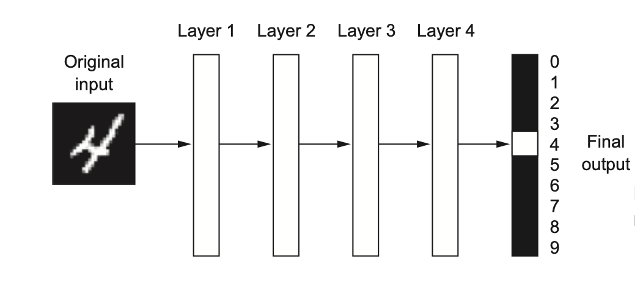
\includegraphics[width=1\textwidth]{1-dl-1}
    \caption{Un Reseau de neurone pour la reconnaissance des caractères.}
    \label{fig:1-dl-1}
\end{figure}

\paragraph{}Comme on peut le voir sur la figure \ref{fig:1-dl-2} , le réseau transforme l'image numérique en représentations de plus en plus différentes de l'image originale et de plus en plus informatives sur le résultat final. On peut  considérer un réseau profond comme une opération de distillation d'informations à plusieurs étapes, où les informations passent par des filtres successifs et sortent de plus en plus purifiées (c'est-à-dire utiles pour certaines tâches).

\begin{figure}[h]
    \centering
    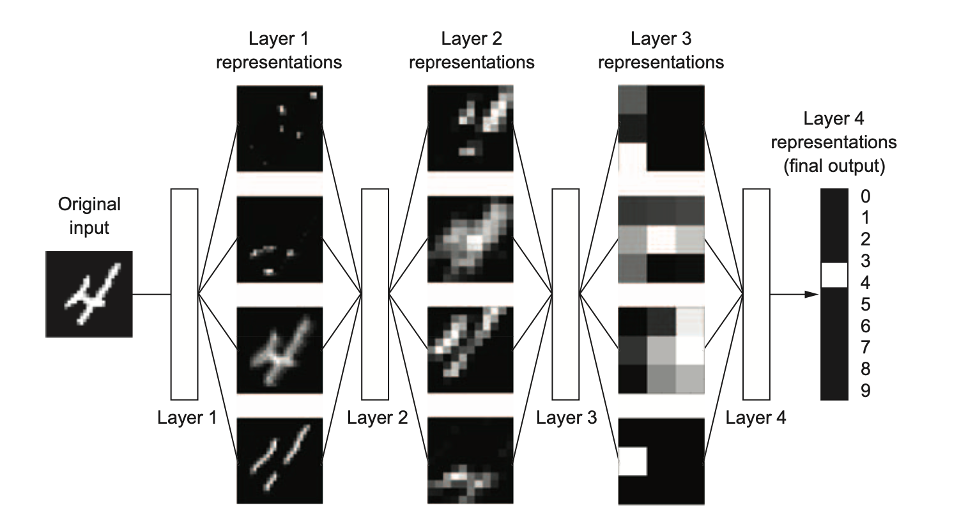
\includegraphics[width=1\textwidth]{1-dl-2}
    \caption{modèle de classification de caractères manuscrits.}
    \label{fig:1-dl-2}
\end{figure}
\paragraph{}

\subsubsection{Fonctionnement}
\paragraph{}La spécification de ce qu'une couche fait à ses données d'entrée est stockée dans les poids de la couche, qui sont essentiellement un ensemble de nombres. En termes techniques, on dirait que la transformation mise en œuvre par une couche est paramétrée par ses poids (voir figure \ref{fig:1-dl-3}). dans  ce contexte, l'apprentissage signifie trouver un ensemble de valeurs pour les pondérations de toutes les couches d'un réseau, de sorte que le réseau mappe correctement les exemples d'entrées sur leurs cibles associées.
Mais voici le problème : un réseau de neurones profonds peut contenir des dizaines de millions de paramètres. Trouver la valeur correcte pour chacun d'eux peut sembler une tâche ardue, d'autant plus que la modification de la valeur d'un paramètre affectera le comportement de tous les autres !
\begin{figure}[h]
    \centering
    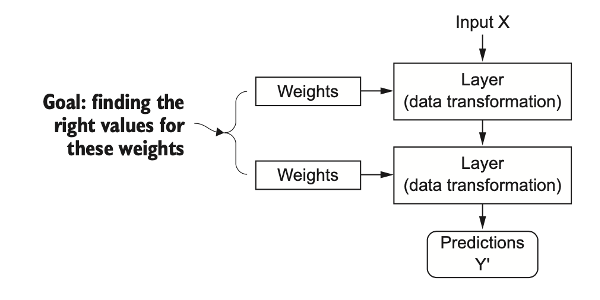
\includegraphics[width=1\textwidth]{1-dl-3}
    \caption{Paramétrisation d’un réseau de neurones}
    \label{fig:1-dl-3}
\end{figure}

\paragraph{}
\paragraph{}

Pour contrôler la sortie d'un réseau de neurones, on doit  être en mesure de mesurer à quelle distance cette sortie (la prédiction, Y’) \cite{dlp}  est de ce que vous attendiez (le résultat attendu, Y). C'est le travail de la fonction de perte du réseau, également appelée fonction objectif. La fonction de perte prend les prédictions du réseau et la véritable cible (ce que vous vouliez que le réseau produise) et calcule un score de distance, capturant la performance du réseau sur cet exemple spécifique (voir figure \ref{fig:1-dl-3}).
\paragraph{}

\begin{figure}[h]
    \centering
    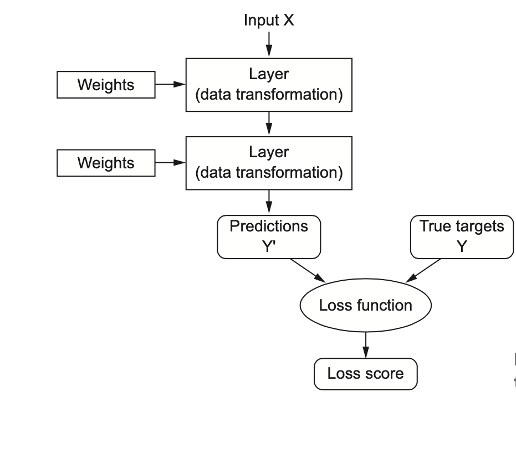
\includegraphics[width=1\textwidth]{1-dl-4}
    \caption{Détermination de la fonction Loss}
    \label{fig:1-dl-4}
\end{figure}

L'astuce fondamentale dans l'apprentissage  profond consiste à utiliser ce score comme un signal de rétroaction pour ajuster un peu la valeur des poids, dans une direction qui abaissera le score de perte pour l'exemple actuel (voir figure \ref{fig:1-dl-5} ). Cet ajustement est le travail de l'optimiseur, qui implémente ce qu'on appelle l'algorithme de rétropropagation : l'algorithme central de l'apprentissage en profondeur. 
\begin{figure}[h]
    \centering
    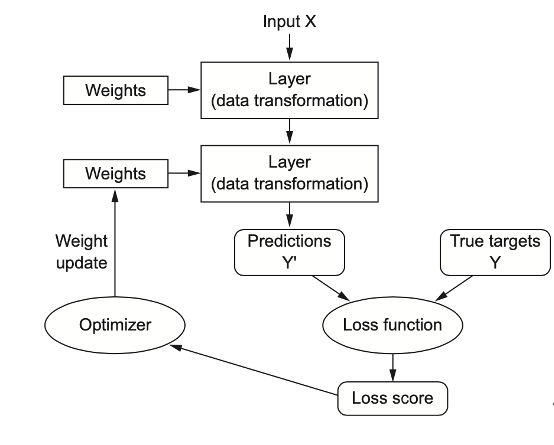
\includegraphics[width=1\textwidth]{1-dl-5}
    \caption{Le Loss Score utilisé pour optimiser le Weigth à  l'entrée}
    \label{fig:1-dl-5}
\end{figure}
\paragraph{}Initialement, les poids du réseau reçoivent des valeurs aléatoires, de sorte que le réseau implémente simplement une série de transformations aléatoires. Naturellement, son rendement est loin de ce qu'il devrait être idéalement, et le score de perte est donc très élevé. Mais avec chaque exemple traité par le réseau, les pondérations sont légèrement ajustées dans la bonne direction et le score de perte diminue. Il s'agit de la boucle d'apprentissage qui, répétée un nombre suffisant de fois (généralement des dizaines d'itérations sur des milliers d'exemples), donne des valeurs de poids qui minimisent la fonction de perte. Un réseau avec une perte minimale est un réseau dont les sorties sont aussi proches que possible des cibles : un réseau entraîné. 
\paragraph{}En résumé, le deep learning implique la collecte et la préparation des données, \cite{dlp}  la construction et l'entraînement du réseau de neurones, l'évaluation du modèle et enfin la prédiction. Le processus de deep learning est souvent itératif, et il peut être nécessaire d'ajuster les paramètres du modèle ou de modifier l'architecture du réseau de neurones pour améliorer les performances du modèle.

\newpage 
\newpage 
\section{deep Learning pour la reconnaissance vocale}

\paragraph{}Dans le domaine de la reconnaissance de locuteur, le Deep Learning est utilisé pour améliorer la précision des systèmes de reconnaissance de la parole en analysant les caractéristiques du signal vocal. Plusieurs méthodes de Deep Learning sont utilisées pour la reconnaissance de locuteur :
\begin{itemize}
    \item \textbf{Réseaux de neurones convolutionnels (CNN)} : Les CNN sont largement utilisés pour l'analyse d'images, mais ils ont également été appliqués à la reconnaissance de locuteur en utilisant des images spectrographiques du signal vocal. Les CNN peuvent extraire des caractéristiques significatives du signal vocal qui peuvent être utilisées pour identifier le locuteur.
    \item \textbf{Réseaux de neurones récurrents (RNN)} : Les RNN sont utilisés pour modéliser des séquences de données, telles que des séquences de phonèmes dans la parole. Les RNN peuvent être utilisés pour identifier le locuteur en analysant les modèles de parole spécifiques à chaque locuteur.
    \item \textbf{Réseaux de neurones profonds (DNN)} : Les DNN sont utilisés pour l'apprentissage en profondeur en utilisant des couches de neurones artificiels. Les DNN ont été utilisés pour la reconnaissance de locuteur en analysant les caractéristiques du signal vocal telles que la fréquence, l'intensité, la durée et les modèles de parole.
    \item \textbf{Réseaux adversaires génératifs (GAN)} : Les GAN sont utilisés pour générer des données synthétiques en imitant les données réelles. Les GAN ont été utilisés pour la reconnaissance de locuteur en générant des images spectrographiques du signal vocal qui peuvent être utilisées pour entraîner des modèles de reconnaissance de locuteur.
\end{itemize}
\paragraph{}Les TDNN (Time-Delay Neural Networks) représentent une architecture de réseaux de neurones artificiels, qui utilisent des couches de neurones à délai temporel pour traiter des données séquentielles ou temporelles. Ces réseaux sont capables de modéliser des dépendances temporelles entre des événements, en prenant en compte l'ordre et le timing des entrées. Les TDNN sont souvent utilisés pour la reconnaissance de la parole, la classification de séries temporelles, la prédiction de séquences, etc.
\paragraph{}En somme, ces techniques et méthodes de Deep Learning permettent d'améliorer la précision de la reconnaissance de locuteur en analysant les caractéristiques du signal vocal de manière plus fine et précise \cite{tdnn}.

\subsection{que représentent les x-vector dans la reconnaissance vocale?}
\paragraph{}Les x-vector sont une représentation numérique de haut niveau d'un segment de signal vocal, qui est utilisée dans la reconnaissance vocale pour l'identification des individus. Les x-vector sont calculés à partir de caractéristiques acoustiques telles que les coefficients cepstraux de fréquence (MFCC) extraits d'un segment de parole \cite{xvectors}.	
\paragraph{}Les x-vector sont généralement extraits en utilisant des réseaux de neurones profonds appelés réseaux de neurones convolutionnels (CNN) et des réseaux de neurones récurrents (RNN), qui sont entraînés à prédire l'identité du locuteur à partir des caractéristiques acoustiques. Le réseau de neurones est ensuite utilisé pour extraire les x-vector à partir de nouvelles données de parole, qui sont ensuite utilisées pour identifier l’individus.
\paragraph{}Les x-vector ont plusieurs avantages par rapport aux méthodes traditionnelles de reconnaissance vocale basées sur les traits acoustiques. Ils peuvent être utilisés pour représenter des segments de parole de longueur variable, sont robustes aux variations de canal et peuvent être utilisés pour l'identification des individus dans des scénarios multi-locuteurs. Les x-vector ont été utilisés avec succès dans de nombreux systèmes de reconnaissance vocale, notamment dans les systèmes de sécurité et de surveillance.

\subsection{que représentent les DNN}

\textbf{Les DNN (Deep Neural Networks)} représentent une classe de modèles de réseaux de neurones artificiels qui sont capables de traiter des données complexes et d'effectuer des tâches de classification, de reconnaissance de motifs, de traitement de langage naturel, etc. Les DNN utilisent plusieurs couches de neurones pour extraire des caractéristiques de plus en plus abstraites à partir des données d'entrée, ce qui leur permet d'apprendre des représentations profondes des données et de réaliser des tâches de manière plus précise et efficace que les modèles de réseaux de neurones plus simples. Les DNN ont trouvé des applications dans de nombreux domaines, notamment la vision par ordinateur, le traitement du langage naturel, la reconnaissance de la parole, la biologie, la médecine, la finance, etc.

\subsection{Les ECAPA-TDNN }
\paragraph{}Les ECAPA-TDNN (Ensemble Classifiers using Adaptive Partitioning Algorithm - Time-Delay Neural Network) sont un type de modèle de classification utilisé en intelligence artificielle et en reconnaissance de formes. Ils combinent les techniques d'ensemble learning (utilisation de multiples classificateurs pour améliorer la précision de la classification) avec les réseaux de neurones à retards temporels (TDNN) pour résoudre des problèmes de classification complexes. Les ECAPA-TDNN sont particulièrement adaptés pour la reconnaissance de formes dans des signaux temporels tels que les signaux audio, les séries chronologiques, les images vidéo, etc. Ils sont largement utilisés dans des domaines tels que la reconnaissance de la parole, la reconnaissance de gestes et la vision par ordinateur \cite{embeddings}.

\subsection{Les ECAPA-TDNN }
\paragraph{}Les PLDA (Probabilistic Linear Discriminant Analysis) sont des modèles d'apprentissage automatique utilisés dans la classification de données. Ils sont principalement utilisés pour l'analyse discriminante linéaire, qui est une méthode statistique qui permet de déterminer la catégorie à laquelle une observation appartient en se basant sur un ensemble de variables prédéfinies. Les PLDA sont souvent utilisés dans le domaine de la reconnaissance vocale pour l'identification des locuteurs, mais peuvent également être appliqués à d'autres types de données. Ils sont considérés comme un outil efficace pour la réduction de dimensionnalité et pour l'analyse des données à grande échelle.

\section{Les bonnes pratiques en matière de reconnaissance vocale}
\paragraph{}Comme pour toute méthode de sécurité, il existe certaines meilleures pratiques de base que les organisations doivent suivre pour s'assurer que les informations de leurs clients ne sont pas en danger \cite{mathworks}.

\begin{itemize}
    \item Établir une méthode d'authentification principale avant toute autre méthode ; cela signifie choisir une forme de validation, qu'il s'agisse d'un code PIN, d'un mot de passe ou d'une biométrie, avant d'accepter d'utiliser plus d'authentifications.
    \item Obtenir le consentement explicite de l'utilisation prévue des utilisateurs pour la mesure de sécurité ; par exemple, accord d'utilisation de la reconnaissance faciale pour permettre les transactions de paiement.
    \item Exiger la méthode d'authentification principale toutes les 72 heures.
    \item Utiliser un pipeline entièrement sécurisé pour toutes les données biométriques et leur manipulation.
    \item Conserver toutes les données biométriques dans un environnement sécurisé et isolé pour empêcher leur acquisition par des fraudeurs.
\end{itemize}
L'utilisation des étapes ci-dessus fournit une excellente base à toute entreprise pour assurer la sécurité des informations de ses clients. Il fournit également une base pour commencer à ajouter plus de niveaux d'authentification afin de créer un système de vérification encore plus puissant.

\section{À quel point la reconnaissance vocale est-elle sécurisée ?}
\paragraph{}La commodité qu'offre la reconnaissance vocale se fait-elle au détriment de la sécurité ? Il y a eu de nombreuses histoires dans les nouvelles sur les pirates capables d'infiltrer les maisons et les entreprises au détriment de leurs propriétaires en utilisant des problèmes de sécurité de reconnaissance vocale. Comme pour toute mesure de sécurité, croire qu'une seule mesure à elle seule est infaillible est imprudent \cite{softjourn}.
\paragraph{}Il reste encore du chemin à parcourir pour parvenir à une identification vocale absolument sécurisée. L'état actuel de la biométrie vocale est vulnérable. Des recherches ont montré que des échantillons de voix provenant de quelque chose comme une vidéo YouTube peuvent être acceptés comme modèles de parole approuvés. Les pirates ont pu enterrer des commandes malveillantes dans du bruit blanc pour contrôler les appareils à commande vocale.
\paragraph{}Selon Lior Atzi, directeur de la gestion des produits chez NICE, deux technologies majeures sont utilisées pour lutter contre la fraude dans l'authentification vocale : la détection de la vivacité et l'authentification continue. 
\paragraph{}La détection de la vivacité, comme son nom l'indique, garantit que l'empreinte digitale ou l'échantillon vocal utilisé est réel. Certaines tentatives pour contrecarrer cette mesure de sécurité sont des voix synthétiques et d'autres implémentations d'intelligence artificielle, mais elles n'ont pas encore suffisamment progressé pour provoquer une menace réelle.
\paragraph{}L'authentification continue vérifie à plusieurs reprises l'identité d'un individu tout au long d'une session, plutôt qu'une seule fois. Cela aide à surmonter les problèmes potentiels tels que les appelants qui changent au milieu d'un appel téléphonique ou d'autres astuces qu'un mauvais acteur pourrait utiliser pour accéder au compte de quelqu'un.


 


\newpage 
\addcontentsline{toc}{section}{Conclusion}
\section*{Conclusion}
\paragraph{}L'authentification vocale rend les connexions aussi simples que parler. Cela peut sembler futuriste, mais c'est la sécurité qui protège les entreprises des violations quotidiennes.
\paragraph{}La reconnaissance vocale est-elle sécurisée ? Oui, la reconnaissance vocale est sécurisée, surtout par rapport aux connexions classiques qui nécessitent un nom d'utilisateur et un mot de passe. Semblable à d'autres biométries, la reconnaissance vocale est plus sécurisée car une personne doit interagir avec un identifiant plutôt que de simplement saisir un code.
\paragraph{}De toute évidence, l'authentification vocale offre de nombreux avantages, tels que des économies de coûts, une sécurité accrue et une expérience client améliorée.
\paragraph{}Cependant, cela vient avec son propre ensemble de défis. Par exemple, parce que la technologie peut être sensible aux bruits et aux signaux parasites.
\paragraph{}Elle reste tout de même un  excellent choix pour accroitre la sécurités des système utilise comme une vérification supplémentaire, car elle ajoute des couches de protection supplémentaires que les codes d'accès manuels pourraient ne pas fournir. L'authentification vocale est bénéfique à la fois pour les clients et pour l'entreprise car elle élimine la frustration associée aux processus de connexion fastidieux.
\paragraph{}La commodité et la sécurité qu'elle offre en font une méthode de vérification dont l'utilisation ne fera qu'augmenter dans tous les secteurs.
\paragraph{}Dans les prochaines décénies, L'authentification par empreinte vocale est susceptible de gagner encore plus en popularité en raison des améliorations de la précision, causées en grande partie par les progrès de l'IA. Cette croissance est également due aux attentes accrues des clients pour un accès rapide et facile à l'information. La biométrie vocale permet un accès rapide, fluide et hautement sécurisé pour une gamme de cas d'utilisation allant des centres d'appels aux applications mobiles et en ligne, en passant par les chatbots, les appareils IoT et l'accès physique.

